% Declare layers
\pgfdeclarelayer{background}
\pgfsetlayers{background,main}

\tikzset{
    in place/.style={
      auto=false,
      fill=white,
      inner sep=2pt,
    },
  }

\tikzstyle{vertex}=[circle,fill=black!25,minimum size=20pt,inner sep=0pt]
\tikzstyle{selected edge} = [draw,line width=5pt,-,red!50]
\tikzstyle{red vertex} = [vertex, fill=red!30, draw=red]
\tikzstyle{blue vertex} = [vertex, fill=blue!30, draw=blue]
\tikzstyle{edge} = [draw,thick,-]
\tikzstyle{diredge} = [draw,thick,->]

\section{Bipartite Graphen}
\begin{frame}{Bipartite Graphen}

\setbeamercovered{invisible}

\begin{figure}
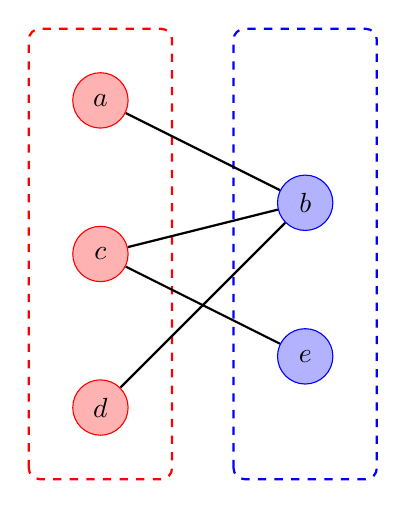
\begin{tikzpicture}[scale=1.3, auto,swap]
	\foreach \pos/\name in {{(0,2)/a}, {(2,1)/b}, {(0,0.5)/c},
                            {(0,-1)/d}, {(2,-0.5)/e}}
        \node[vertex] (\name) at \pos {$\name$};
    \foreach \source/ \dest in {a/b, c/e, d/b, c/b}
        \path[edge] (\source) -- (\dest);
    
	\begin{pgfonlayer}{background}
		    \pause
        \draw [red, rounded corners,thick, dashed] (-0.7,-1.7) rectangle (0.7,2.7);
        \draw [blue, rounded corners,thick, dashed] (1.3,-1.7) rectangle (2.7,2.7);
    \end{pgfonlayer}    
    
    \foreach \vertex in {a, c, d}
        \path<3-> node[red vertex] at (\vertex) {$\vertex$};
    \foreach \vertex in {b,e}
        \path<3-> node[blue vertex] at (\vertex) {$\vertex$};

	
\end{tikzpicture}
\end{figure}
\end{frame}

\subsection{Matchings}
\begin{frame}{Matchings}
\setbeamercovered{invisible}
\begin{block}{Definition}
Sei \(G = (V, E), \ E \subseteq \set{\set{u, v} \given u, v \in V}\) ein ungerichteter Graph.\\ \pause Eine Menge von Kanten \(M \subseteq E\) hei\ss{}t \textbf{Matching}\pause, falls
\[
\forall e_1,e_2 \in M: e_1 \neq e_2 \Rightarrow e_1 \cap e_2 = \varnothing.
\]\pause
\(M \in \mathcal{M} \defas \set{M \subseteq E \given \text{\(M\) ist Matching}}\) hei\ss{}t \textbf{inklusionsmaximal}\pause, falls
\[
\forall M' \in \mathcal{M}: M \subseteq M' \Rightarrow M = M'.
\]\pause
\(M \in \mathcal{M}\) hei\ss{}t \textbf{kardinalit"atsmaximal}\pause, falls
\[
\forall M' \in \mathcal{M}: |M| \geq |M'|
\]\pause
F"ur \(G\) bipartit: \enquote{Maximum Cardinality Bipartite Matching}, kurz \textbf{MCBM}.
\end{block}
\end{frame}

\begin{frame}{Matchings}
\setbeamercovered{invisible}

\begin{figure}
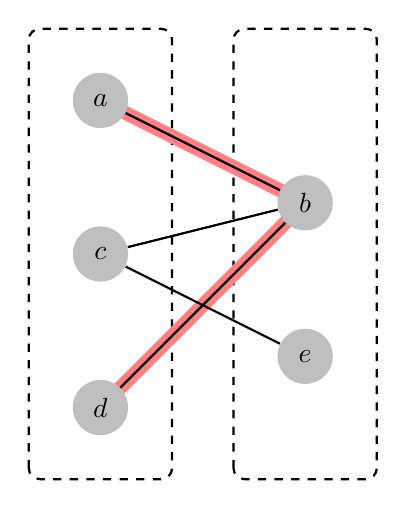
\begin{tikzpicture}[scale=1.3, auto,swap]
	\foreach \pos/\name in {{(0,2)/a}, {(2,1)/b}, {(0,0.5)/c},
                            {(0,-1)/d}, {(2,-0.5)/e}}
        \node[vertex] (\name) at \pos {$\name$};
    \foreach \source/ \dest in {a/b, c/e, d/b, c/b}
        \path[edge] (\source) -- (\dest);
    
	\begin{pgfonlayer}{background}
        \draw [black, rounded corners,thick, dashed] (-0.7,-1.7) rectangle (0.7,2.7);
        \draw [black, rounded corners,thick, dashed] (1.3,-1.7) rectangle (2.7,2.7);
        \pause
        \foreach \source / \dest in {a/b,d/b}
            \path[selected edge] (\source.center) -- (\dest.center);
    \end{pgfonlayer}
\end{tikzpicture}
\pause\caption*{\large \textbf{Kein} Matching}
\end{figure}
\end{frame}

\begin{frame}{Matchings}
\setbeamercovered{invisible}

\begin{figure}
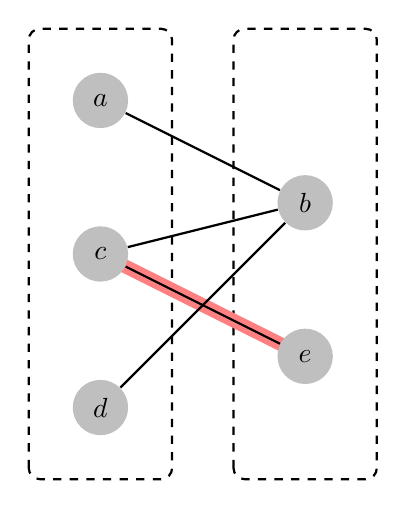
\begin{tikzpicture}[scale=1.3, auto,swap]
	\foreach \pos/\name in {{(0,2)/a}, {(2,1)/b}, {(0,0.5)/c},
                            {(0,-1)/d}, {(2,-0.5)/e}}
        \node[vertex] (\name) at \pos {$\name$};
    \foreach \source/ \dest in {a/b, c/e, d/b, c/b}
        \path[edge] (\source) -- (\dest);
    
	\begin{pgfonlayer}{background}
        \draw [black, rounded corners,thick, dashed] (-0.7,-1.7) rectangle (0.7,2.7);
        \draw [black, rounded corners,thick, dashed] (1.3,-1.7) rectangle (2.7,2.7);
        \foreach \source / \dest in {c/e}
            \path[selected edge] (\source.center) -- (\dest.center);
    \end{pgfonlayer}
\end{tikzpicture}
\pause\caption*{\large Matching, aber weder inklusions- noch kardinalit"atsmaximal}
\end{figure}
\end{frame}

\begin{frame}{Matchings}
\setbeamercovered{invisible}

\begin{figure}
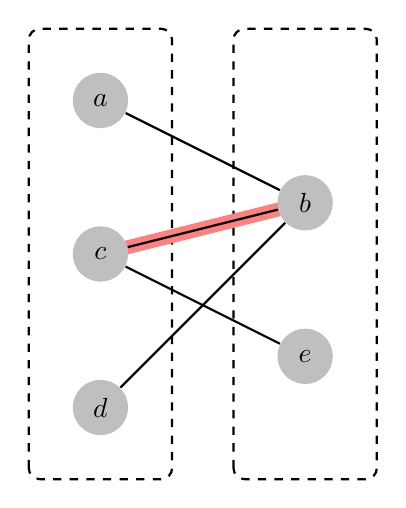
\begin{tikzpicture}[scale=1.3, auto,swap]
	\foreach \pos/\name in {{(0,2)/a}, {(2,1)/b}, {(0,0.5)/c},
                            {(0,-1)/d}, {(2,-0.5)/e}}
        \node[vertex] (\name) at \pos {$\name$};
    \foreach \source/ \dest in {a/b, c/e, d/b, c/b}
        \path[edge] (\source) -- (\dest);
    
	\begin{pgfonlayer}{background}
        \draw [black, rounded corners,thick, dashed] (-0.7,-1.7) rectangle (0.7,2.7);
        \draw [black, rounded corners,thick, dashed] (1.3,-1.7) rectangle (2.7,2.7);
        \foreach \source / \dest in {c/b}
            \path[selected edge] (\source.center) -- (\dest.center);
    \end{pgfonlayer}
\end{tikzpicture}
\pause\caption*{\large Inklusions-, aber nicht kardinalit"asmaximales Matching}
\end{figure}
\end{frame}

\begin{frame}{Matchings}
\setbeamercovered{invisible}

\begin{figure}
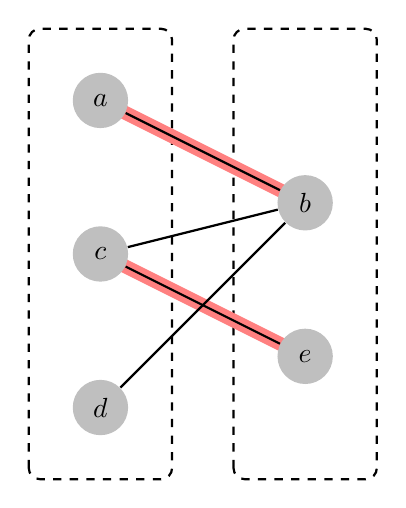
\begin{tikzpicture}[scale=1.3, auto,swap]
	\foreach \pos/\name in {{(0,2)/a}, {(2,1)/b}, {(0,0.5)/c},
                            {(0,-1)/d}, {(2,-0.5)/e}}
        \node[vertex] (\name) at \pos {$\name$};
    \foreach \source/ \dest in {a/b, c/e, d/b, c/b}
        \path[edge] (\source) -- (\dest);
    
	\begin{pgfonlayer}{background}
        \draw [black, rounded corners,thick, dashed] (-0.7,-1.7) rectangle (0.7,2.7);
        \draw [black, rounded corners,thick, dashed] (1.3,-1.7) rectangle (2.7,2.7);
        \foreach \source / \dest in {a/b, c/e}
            \path[selected edge] (\source.center) -- (\dest.center);
    \end{pgfonlayer}
\end{tikzpicture}
\pause\caption*{\large Kardinalit"atsmaximales Matching}
\end{figure}
\end{frame}

\begin{frame}{Complete Prime Pairing}
\setbeamercovered{invisible}
\begin{block}{Definition}\pause
Ein \textbf{Complete Prime Pairing} einer Menge \(\varnothing \neq A \subseteq \mathbb{N}\) ist eine selbstinverse, fixpunktfreie Abbildung \(f\colon A \to A\), sodass \(\forall a \in A: a + f(a) \in \mathbb{P}\).
\end{block}

\pause\begin{block}{Problem}
Gegeben eine Liste \(N\) von nat"urlichen Zahlen und \(a, b \in N \ (a \neq b)\), existiert ein Complete Prime Pairing von N, in dem \(a\) und \(b\) gepaart werden?\\ \pause
\begin{itemize}
\item Falls \(a+b\notin \mathbb{P}\), gebe \enquote{Nein} aus.\pause\ Ansonsten entferne \(a, b\) aus \(N\).\pause
\item Setze \(V_1 \defas \set{v\in N \given \text{$v$ gerade}}, V_2 \defas N \setminus V_1\).\pause
\item Setze \(V \defas N\) und \(E \defas \set{\set{a,b}\given a,b\in N \text{ und } a+b\in \mathbb{P}}\). Dann ist \(G \defas (V, E)\) bipartit.\pause
\item Berechne ein MCBM \(M\) von \(G\) und gebe \enquote{Ja} aus, falls \(|M| = |V_1| = |V_2|\).
\end{itemize}
\end{block}
\end{frame}

\subsection{MCBM mit Max-Flow}

\begin{frame}{MCBM mit Max-Flow}
\setbeamercovered{invisible}
\begin{figure}
\begin{tikzpicture}[scale=1.3, auto,swap]
	\foreach \pos/\name in {{(0,2)/a}, {(2,1)/b}, {(0,0.5)/c},
                            {(0,-1)/d}, {(2,-0.5)/e}}
        \node[vertex] (\name) at \pos {$\name$};
    \foreach \source/ \dest in {a/b, c/e, d/b, c/b}
        \path[edge] (\source) -- (\dest);

	\foreach \source/ \dest/ \fr in {s/a/3, s/c/3, s/d/3, b/t/4, e/t/4}
		\path<\fr->[diredge, dashed] (\source) -- node[pos=0.6, in place] {$1$} (\dest); 
    
    \pause
    \foreach \source/ \dest/ \pos in {a/b/0.5, c/e/0.7, d/b/0.7, c/b/0.5}
        \path[diredge] (\source) -- node[pos=\pos, in place] {$1$} (\dest);
    
	\pause\node[vertex, draw=black] (s) at (-2,0.5) {$s$};
	\pause\node[vertex, draw=black] (t) at (4,0.5) {$t$};
    
	\begin{pgfonlayer}{background}
        \foreach \source / \dest in {s/a, a/b, b/t, s/c, c/e, e/t}
            \path<5->[selected edge] (\source.center) -- (\dest.center);
    \end{pgfonlayer}
\end{tikzpicture}
\end{figure}
\end{frame}

\subsection{Augmenting Paths}

\begin{frame}{MCBM mit Augmenting Paths}
\setbeamercovered{invisible}
\begin{block}{Augmenting Paths}
Sei \(G = (V,E), \ V = V_1 \dot{\cup} V_2\) bipartit und \(M \subseteq E\) ein Matching.\pause

Ein Pfad \((v_1,...,v_n)\) in \(G\) hei\ss{}t \textbf{Augmenting Path} (in G bzgl. M)\pause, falls
\begin{itemize}
\item \(v_1 \in V_1 \setminus \bigcup M\) (freier Knoten links)\pause
\item \(\forall i \in \set{1,...,n-1}: \set{v_i,v_i+1} \in
\begin{cases*}
	E \setminus M, & $i$ ungerade,\\
	M, & $i$ gerade.
\end{cases*}\)\pause
\item \(v_n \in V_2 \setminus \bigcup M\) (freier Knoten rechts)
\end{itemize}
\end{block}
\end{frame}

\begin{frame}{MCBM mit Augmenting Paths}
\setbeamercovered{invisible}
\begin{block}{Lemma von Claude Berge}
Sei \(G = (V,E)\) bipartit und \(M \subseteq E\) ein Matching. \pause Dann ist M kardinalit"atsmaximal, genau dann wenn kein Augmenting Path in G bzgl. M existiert.
\end{block}\pause
\begin{block}{Beweisidee}\pause
Ist \(M\) ein Matching und \((v_1,...,v_n)\) ein Augmenting Path\pause, so ist
\[
M' \defas M \setminus P \cup P \setminus M, \text{ wobei } P \defas \set{\set{v_i, v_{i+1}} \given i \in \set{1,...,n-1}}
\]
(flippe die Kanten entlang des Pfades) ein Matching mit \(|M'| = |M| + 1\).
\end{block}
\end{frame}

\begin{frame}{MCBM mit Augmenting Paths}
\setbeamercovered{invisible}
\begin{block}{Augmenting Path Algorithmus}
Gegeben: bipartiter Graph \(G = (V, E)\).
\begin{itemize}
\pause\item[(1)] Initialisiere \(M \defas \varnothing\).
\pause\item[(2)] Suche (greedy) einen Augmenting Path. Gebe \(M\) aus, falls keinen gefunden.
\pause\item[(3)] Flippe die Kanten entlang des gefundenen Pfades. Gehe zu (2).
\end{itemize}\pause
Findet MCBM in Laufzeit \(O(|V|\cdot |E|)\).
\end{block}
\end{frame}

\begin{frame}{MCBM mit Augmenting Paths}
\setbeamercovered{invisible}

\begin{figure}
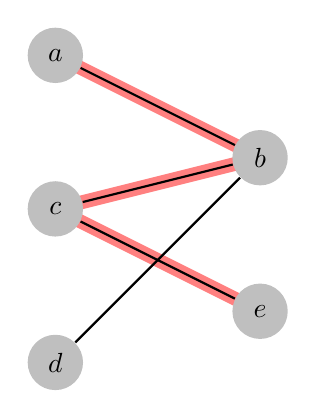
\begin{tikzpicture}[scale=1.3, auto,swap]
	\foreach \pos/\name in {{(0,2)/a}, {(2,1)/b}, {(0,0.5)/c},
                            {(0,-1)/d}, {(2,-0.5)/e}}
        \node[vertex] (\name) at \pos {$\name$};
    \foreach \source/ \dest in {a/b, c/e, d/b, c/b}
        \path[edge] (\source) -- (\dest);
    
	\begin{pgfonlayer}{background}
        \foreach \source / \dest/ \fr in {c/b/2, a/b/3, c/e/3}
            \path<\fr>[selected edge] (\source.center) -- (\dest.center);
    \end{pgfonlayer}
\end{tikzpicture}
\end{figure}
\end{frame}

%\begin{block}{Block 1}
%\begin{itemize}
%\item Bullet point 1
%\pause
%\item Bullet point 2
%\item \dots
%\end{itemize}
%\end{block}
